\documentclass[12pt, a4paper]{ntut-report}
\usepackage[dvips,xetex]{graphicx}
\usepackage{ifpdf,mla}% <-- mla.sty requires ifpdf.sty, but (perversely) doesn't load it
%\usepackage{fontspec}
\usepackage{geometry}
\usepackage{lipsum}
\usepackage{xeCJK}
\usepackage{wallpaper}
\usepackage{pdfpages}
\usepackage{indentfirst}
\usepackage{setspace}
\usepackage{hyperref}
\usepackage{zhnumber}
\usepackage{titlesec}
\usepackage{amsmath}
\usepackage[backend=bibtex,sorting=none]{biblatex}   

\renewcommand{\baselinestretch}{1.5}
\xeCJKsetup{AutoFakeBold=true, AutoFakeSlant=true}
\setCJKmainfont{標楷體} % 中文字體
\setmainfont{Times New Roman} % 英文字體
\geometry{a4paper,total={297mm,210mm},top=4.5cm,bottom=0.75cm,left=2.5cm,right=2.2cm} % 頁面設定,不需修改
\pagestyle{plain} % 頁碼
\addbibresource{reference.bib}

%
% this file is encoded in utf-8
%

%% 這些設定值將會用於呈現在首頁上,請進行填入
%% Please fill in the information which will be shown on the cover and in the abstract. All Chinese and English information must be matched to each other. If you don’t have any Chinese information, please skip the Chinese ones, but all English Information is required.

%
% 中文論文設定值,請根據以下的範例進行填入
%

% 論文題目(中文)
% Thesis Title (Chinese)
% \newcommand\cTitle{待訂}

% 我的姓名(中文)
% My Name(Chinese)
\newcommand\myCname{周玟萱}

% 指導教授的姓名 (中文),使用頓號隔開 
% Advisor (Chinese), use “、” to separate names
\newcommand\advisorCname{陳香君 博士}

% 校名 (中文)
% School Name(Chinese)
\newcommand\univCname{國立臺北科技大學}

% 系所名 (中文)
% Department Name(Chinese)
\newcommand\deptCname{創新資安碩士班}

% 學位名 (中文)
% Degree Name(Chinese)
\newcommand\degreeCname{碩士}

% 口試年份 (中文、民國)
% Year of Oral Defense(Chinese)
\newcommand\cYear{一百一十四}

% 口試月份 (中文)
% Month of Oral Defense(Chinese)
\newcommand\cMonth{五}

% 畢業學年度 (中文)
% 如 112 學年度第2學期畢業,當時為民國113年6月,學年度即為112,不是113。
\newcommand\cAcademicYear{一百一十三}

% 畢業學期(中文)
% Academic Year (Chinese)
\newcommand\cGraduateSemester{二}

%
% 英文論文設定值,請根據以下的範例進行填入
%

% 論文題目 (英文)
% Thesis Title (Engslih)
\newcommand\eTitle{S2GE-NIDS: A hybrid architecture combining structured semantics and generation embedded network intrusion detection system in IoT}

% 我的姓名(英文)
% My Name(English)
\newcommand\myEname{Wen-Hsuan, Chou}

% 指導教授的姓名 (英文),使用逗號隔開
% 例如:Dr. Kuo Jong-Yi, Dr. A B-C, ...
%
% Advisor (Ensligh), use “, ” to separate names
% e.g. Dr. Kuo Jong-Yi, Dr. A B-C, ...
\newcommand\advisorEname{Shiang-Jiun Chen, Ph.D.}

% 校名(英文)
% School Name(English)
\newcommand\univEname{National Taipei University of Technology}

% 系所全名 (英文)
% Department Name(English)
\newcommand\fulldeptEname{Department of Science in Information Security}

\newcommand\deptEname{Science in Information Security}

% 學位名 (英文)
% Degree(English)
\newcommand\degreeEname{Master of Science in Information Security}

% 口試年份 (阿拉伯數字、西元)
% Year of Oral Defense(English)
\newcommand\eYear{2025}

% 口試月份 (英文)
% Month of Oral Defense(English)
\newcommand\eMonth{May}

%畢業級別;用於書背列印;若無此需要可忽略
\newcommand\GraduationClass{113}

%%%%%%%%%%%%%%%%%%%%%%

\begin{document}

% 封面、不用浮水印 Cover without a watermark
\begin{titlepage}
    \newpage
    \begin{center}
        % 北科的 Logo
        
\includegraphics[width=13cm]{ntut-logo-with-label.png}
        
        % 北科的系所名與學位名,以換行隔開
        \huge\bf\deptCname\\% 系所名
        \huge\bf\degreeCname 學位論文\\% 學位名
        % \huge\bf\fulldeptEname \\% 系所英文名
        % \huge\bf\degreeEname Thesis \\ % “Master Thesis” or “Ph.D. Dissertation”

        % 中文與英文論文名稱
        % 如果你不需要英文,你可以註解 \eTitle
        \vfill
        \huge\bf\cTitle\\ %%%%%
        \LARGE\bf\eTitle\\ %%%%%

        % 研究生(中文)
        \vfill
        {\Large 研究生:\myCname}
        %  {\Large Researcher: \myEname}

        % 指導老師(中文)
        \vfill
        {\Large 指導教授:\advisorCname}
        % {\Large Advisor: \advisorEname}

        % 畢業年份(中文)
        \vfill
        {\Large 中華民國{\cYear 年}{\cMonth 月}}
        %  {\Large \eMonth, \eYear}
    \end{center}
\end{titlepage}
% 留白頁、不用浮水印 Blank page without a watermark
\newpage
\thispagestyle{empty}
\null
\newpage

% 新增浮水印 Add Watermarks
\CenterWallPaper{.64}{ntut-logo.png}

% 封面、要浮水印 Cover with a watermark
\begin{titlepage}
    \newpage
    \begin{center}
        % 北科的 Logo
        
\includegraphics[width=13cm]{ntut-logo-with-label.png}
        
        % 北科的系所名與學位名,以換行隔開
        \huge\bf\deptCname\\% 系所名
        \huge\bf\degreeCname 學位論文\\% 學位名
        % \huge\bf\fulldeptEname \\% 系所英文名
        % \huge\bf\degreeEname Thesis \\ % “Master Thesis” or “Ph.D. Dissertation”

        % 中文與英文論文名稱
        % 如果你不需要英文,你可以註解 \eTitle
        \vfill
        \huge\bf\cTitle\\ %%%%%
        \LARGE\bf\eTitle\\ %%%%%

        % 研究生(中文)
        \vfill
        {\Large 研究生:\myCname}
        %  {\Large Researcher: \myEname}

        % 指導老師(中文)
        \vfill
        {\Large 指導教授:\advisorCname}
        % {\Large Advisor: \advisorEname}

        % 畢業年份(中文)
        \vfill
        {\Large 中華民國{\cYear 年}{\cMonth 月}}
        %  {\Large \eMonth, \eYear}
    \end{center}
\end{titlepage}
% 「學位論文口試委員會審定書」掃描檔,請檢附完整簽名之審定書掃描檔
% Please add "Oral Defense Committee Signature Form" with complete signatures.
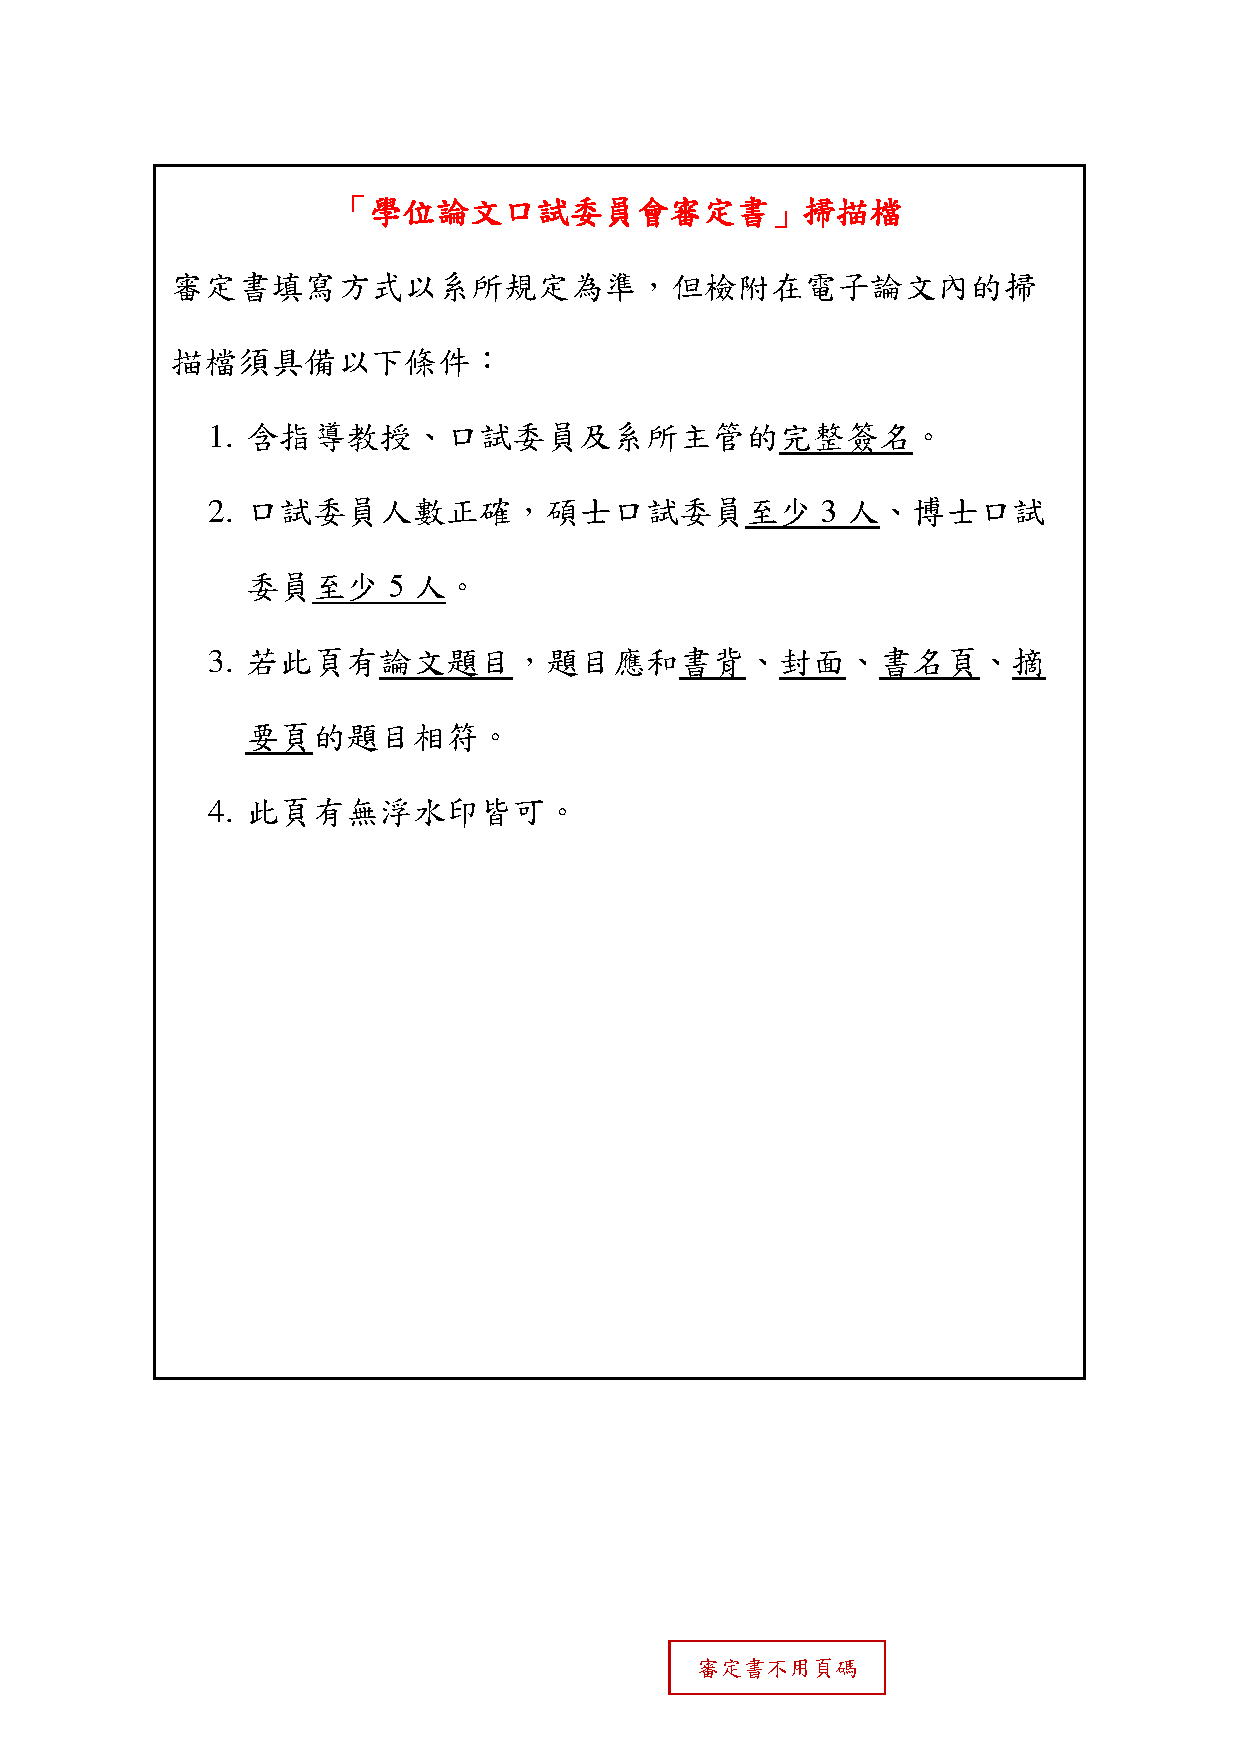
\includepdf[pages=-]{static-page/signpage.pdf}

\pagenumbering{roman}

% 摘要頁(中文)Abstract (Chinese)
% If you don’t have Chinese abstract, please delete this one.
% 中文摘要頁
\begin{ZhAbstract}
    \begin{ZhAbstractItems}
        % 論文名稱,請在 ntut-labels.tex 定義
        \noindent \text 論文名稱:\cTitle

        % 論文頁數,請自己填
        \noindent \text 頁數:(請自己填)頁

        % 校所別,請在 ntut-labels.tex 定義
        \noindent \text 校所別:\univCname \space \deptCname

        % 畢業時間,請在 ntut-labels.tex 定義
        \noindent \text 畢業時間:\cAcademicYear 學年度 \space 第\cGraduateSemester 學期

        % 學位,請在 ntut-labels.tex 定義
        \noindent \text 學位:\degreeCname

        % 研究生,請在 ntut-labels.tex 定義
        \noindent \text 研究生:\myCname

        % 指導教授,請在 ntut-labels.tex 定義
        \noindent \text 指導教授:\advisorCname

        % 關鍵詞,請自己填,請自己填,多個關鍵字以逗號(、)隔開
        \noindent \text 關鍵詞:(請自己填)

    \end{ZhAbstractItems}

    \begin{ZhAbstractDescription}
        摘要為論文或報告的精簡概要,其目的是透過簡短的敘述使讀者大致瞭解整篇報告的內容。摘要的內容通常須包括問題的描述以及所得到的結果,但以不超過 500 字或一頁為原則,且不得有參考文獻或引用圖表等。以中文撰寫之論文除中文摘要外,得於中文摘要後另附英文摘要。標題使用 20pt 粗標楷體並於上、下方各空一行(1.5 倍行高,字型 12pt 空行)後鍵入摘要內容。摘要頁須編頁碼(小寫羅馬數字表示頁碼)。
    \end{ZhAbstractDescription}
    
\end{ZhAbstract}


% 摘要頁(英文)Abstract (English)
% 英文摘要頁
\begin{EnAbstract}
    \begin{EnAbstractItems}
        % 論文名稱,請在 ntut-labels.tex 定義
        \noindent \text Title: \eTitle

        % 論文總頁數,同最後一頁阿拉伯數字頁碼
        % Page number, same as the page number of the last page, not the total pages in pdf file.
        \noindent \text Pages: (Fill it)

        % 校所別,請在 ntut-labels.tex 定義
        \noindent \text School: \univEname

        % 系所別,請在 ntut-labels.tex 定義
        \noindent \text Department: \deptEname

        % 畢業時間,請在 ntut-labels.tex 定義
        \noindent \text Time: \eMonth, \eYear

        % 學位,請在 ntut-labels.tex 定義
        \noindent \text Degree: \degreeEname

        % 研究生,請在 ntut-labels.tex 定義
        \noindent \text Researcher: \myEname

        % 指導教授,請在 ntut-labels.tex 定義
        \noindent \text Advisor: \advisorEname
        
        % 關鍵詞,請自己填,多個關鍵字以逗號 "," 隔開
        \noindent \text Keyword: (Fill it)

    \end{EnAbstractItems}

    \begin{EnAbstractDescription}
        Start writing abstract from here. Start writing abstract from here. Start writing abstract from here. Start writing abstract from here. Start writing abstract from here. Start writing abstract from here. Start writing abstract from here. Start writing abstract from here.
    \end{EnAbstractDescription}
    
\end{EnAbstract}


% 鳴謝 Acknowledgements
\begin{Thanks}
    所有對於研究提供協助之人或機構,作者都可在誌謝中表達感謝之意。
\end{Thanks}
% 目錄、表目錄與圖目錄 Table of Contents, List of tables, List of figures
\begin{TableOfContent}
    \tableofcontents
\end{TableOfContent}

\begin{TableOfContent}
    \listoffigures
\end{TableOfContent}

\begin{TableOfContent}
    \listoftables
\end{TableOfContent}
 
\pagenumbering{arabic}

% 章節一 Chapter 1
\begin{ZhChapter}

\chapter{Introduction}

After several decades of development, deep learning \cite{deepLearning} technology has achieved significant breakthroughs in the last ten years, largely due to the remarkable improvements in GPU computational power. Consequently, the predictive and analytical capabilities of models have achieved substantial advancements. Numerous models have been launched by major companies and applied in practical scenarios, leading to significant changes in our daily lives.

The model training process can be broadly divided into several key steps: collecting data and organizing it into datasets, partitioning the datasets into training and validation sets as needed, initializing model parameters, evaluating the performance of the model, adjusting the model parameters, and repeating the training until the target is achieved or computational resources are exhausted. During the evaluation of the model's performance, we use a function called the loss function. Its purpose is to calculate the difference between the model's predicted results and the ground truth, which helps model adjust its parameter to better fit the target. Therefore, different loss functions can influence the direction of model adjustments, significantly impacting the final outcomes of the model.

However, the design of a loss function is often closely related to the propose of the model. In other words, different models may require experts from specific fields to assist in designing the loss function to enhance the speed and effectiveness of model training. Nevertheless, recent research has shown that it’s feasible to use Genetic Programming (GP) to automatically generate loss functions. Due to the domain-independent nature of GP, it allows us to develop an algorithm that can automatically create the required loss function without needing specialized knowledge in that particular field. However, this method typically requires a significant amount of time and computational resources.

Given the rapid flow of information in today's society, we often need a quick way to find the necessary loss function to optimize the training process of the model. This paper proposes an efficiency-oriented GP algorithm, aiming to reduce the time required for GP to search for the optimal algorithm while maintaining the same level of effectiveness.

The structure of this paper is as follows: Chapter 2 is related work. This chapter provides a detailed illustration to the development and history of Genetic Programming (GP), the detailed description of the loss function and how they collaborate with deep learning model, and how loss functions are randomly generated via genetic programming. Chapter 3 is proposed algorithm and main methodology. In this chapter, we will explain the architecture of the algorithm implemented in this paper. After that, we will then describe the experimental environment setup and the initial parameter values. Finally, we will present the methods and procedures used in this paper. Chapter 4 is results analysis. This section will show the detail parameter settings among all compared peer-algorithm. After that, we will present the analysis of the results by organizing the experimental results into charts and figures. Finally, we will explain the outcomes and analyze why our algorithm can achieve the similar result while decreasing the usage of computational resources. Chapter 5 is conclusion and future work. In this chapter, we will provide the conclusion of this paper by outlining the contribution we have made so far. After that, we would like to discuss potential directions for future research or possible way to apply this algorithm in practical.
% \section{研究動機與背景(小標)}

% \begin{equation} 
%     \mbox{$x = \dfrac{-b\pm\sqrt{b^2-4ac}}{2a}$}
% \end{equation}

% \subsection{研究背景(小小標)}

% \text 背景內文背景內文背景內文背景內文,背景內文背景內文背景內文背景內文背景內文背景內文,如表 1.1 所示。

% \begin{table*}[htbp]
%     \centering
%     \caption{表格範例標題} \label{tab: complexity}
%     \makebox[\linewidth][c]{
%     \renewcommand\arraystretch{1.2}{
%         \begin{tabular}{| l | c  c  c  c |}
%         \hline
%         Protocol & $P$ & $CS_1$ & $CS_2$ & $RG$ \\
%         \hline
%         SD & $O(1)$, $O(1)$, N/A & $O(n-t)$, $O(1)$, N/A & $O(n-t)$, $O(1)$, N/A & $O(1)$, $O(n)$, $O(n)$ \\
%         MSSMul & $O(1)$, $O(1)$, N/A & $O(n-t)$, $O(n)$, $O(1)$ & $O(n-t)$, $O(n)$, N/A & $O(1)$, $O(n)$, $O(n)$ \\
%         MSSAdd & $O(1)$, $O(1)$, N/A & $O(n-t)$, $O(n)$, $O(1)$ & N/A, N/A, N/A & $O(1)$, $O(n)$, $O(n)$ \\
%         SC & $O(1)$, $O(1)$, N/A & $O(n-t)$, $O(n)$, $O(1)$ & $O(n-t)$, $O(n)$, N/A & $O(1)$, $O(n)$, $O(n)$ \\
%         \hline 
%         \end {tabular}
%     }}
% \end {table*}

% \subsubsection{研究動機(小小標)}

% \begin{equation} 
%     \mbox{$(1+x)^n = 1 + \dfrac{nx}{1!} + \dfrac{n(n-1)x^2}{2!}$}
% \end{equation}

% 動機動機動機動機,動機動機動機動機動機動機動機動機動機動機動機動機,動機動機動機動機動機動機動機動機。

% 動機動機動機動機動機動機動機動機,動機動機動機動機動機動機動機動機動機動機動機動機。動機動機動機動機動機動機動機動機,動機動機動機動機動機動機動機動機動機動機動機動機。動機動機動機動機動機動機動機動機,動機動機動機動機動機動機動機動機動機動機動機動機,如圖 1.1、圖 1.2 所示。

% \begin{figure*}[htbp]
%     \centering
%     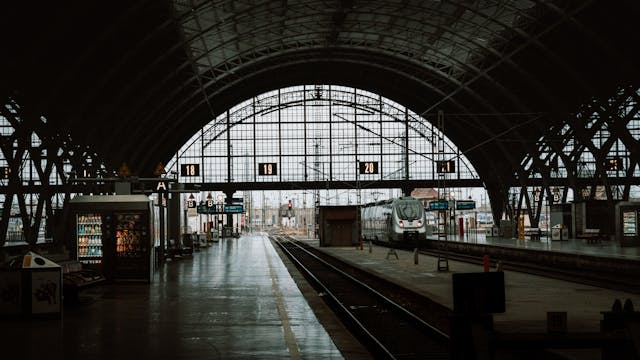
\includegraphics[width = 1\textwidth]{image.jpeg}
%     \caption{Cool train station}
%     \label{fig: image}
% \end{figure*}

% \begin{figure*}[htbp]
%     \centering
%     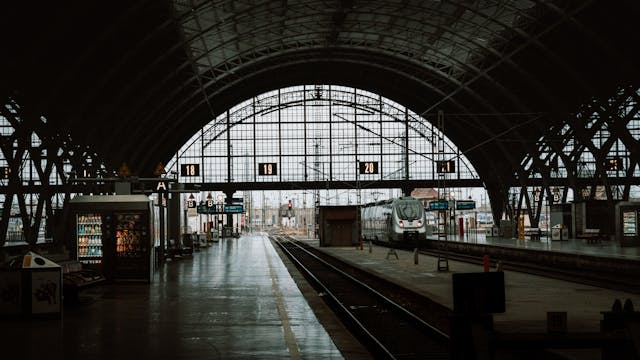
\includegraphics[width = 1\textwidth]{image.jpeg}
%     \caption{Cool train station}
%     \label{fig: image}
% \end{figure*}

% \begin{table*}[htbp]
%     \centering
%     \caption{表格範例標題} \label{tab: complexity}
%     \makebox[\linewidth][c]{
%     \renewcommand\arraystretch{1.2}{
%         \begin{tabular}{| l | c  c  c  c |}
%         \hline
%         Protocol & $P$ & $CS_1$ & $CS_2$ & $RG$ \\
%         \hline
%         MSSMul & $O(1)$, $O(1)$, N/A & $O(n-t)$, $O(n)$, $O(1)$ & $O(n-t)$, $O(n)$, N/A & $O(1)$, $O(n)$, $O(n)$ \\
%         MSSAdd & $O(1)$, $O(1)$, N/A & $O(n-t)$, $O(n)$, $O(1)$ & N/A, N/A, N/A & $O(1)$, $O(n)$, $O(n)$ \\
%         SC & $O(1)$, $O(1)$, N/A & $O(n-t)$, $O(n)$, $O(1)$ & $O(n-t)$, $O(n)$, N/A & $O(1)$, $O(n)$, $O(n)$ \\
%         MSSMul & $O(1)$, $O(1)$, N/A & $O(n-t)$, $O(n)$, $O(1)$ & $O(n-t)$, $O(n)$, N/A & $O(1)$, $O(n)$, $O(n)$ \\
%         MSSAdd & $O(1)$, $O(1)$, N/A & $O(n-t)$, $O(n)$, $O(1)$ & N/A, N/A, N/A & $O(1)$, $O(n)$, $O(n)$ \\
%         SC & $O(1)$, $O(1)$, N/A & $O(n-t)$, $O(n)$, $O(1)$ & $O(n-t)$, $O(n)$, N/A & $O(1)$, $O(n)$, $O(n)$ \\
%         \hline 
%         \end {tabular}
%     }}
% \end {table*}

% 動機動機動機動機,動機動機動機動機動機動機動機動機動機動機動機動機,動機動機動機動機動機動機動機動機。

% 動機動機動機動機,動機動機動機動機動機動機動機動機動機動機動機動機,動機動機動機動機動機動機動機動機。動機動機動機動機,動機動機動機動機動機動機動機動機動機動機動機動機,動機動機動機動機動機動機動機動機。

% 動機動機動機動機,動機動機動機動機動機動機動機動機動機動機動機動機,動機動機動機動機動機動機動機動機。動機動機動機動機,動機動機動機動機動機動機動機動機動機動機動機動機,動機動機動機動機動機動機動機動機。動機動機動機動機,動機動機動機動機動機動機動機動機動機動機動機動機,動機動機動機動機動機動機動機動機。

% 動機動機動機動機,動機動機動機動機動機動機動機動機動機動機動機動機,動機動機動機動機動機動機動機動機。動機動機動機動機,動機動機動機動機動機動機動機動機動機動機動機動機,動機動機動機動機動機動機動機動機。動機動機動機動機,動機動機動機動機動機動機動機動機動機動機動機動機,動機動機動機動機動機動機動機動機。動機動機動機動機,動機動機動機動機動機動機動機動機動機動機動機動機,動機動機動機動機動機動機動機動機。

% \begin{figure*}[htbp]
%     \centering
%     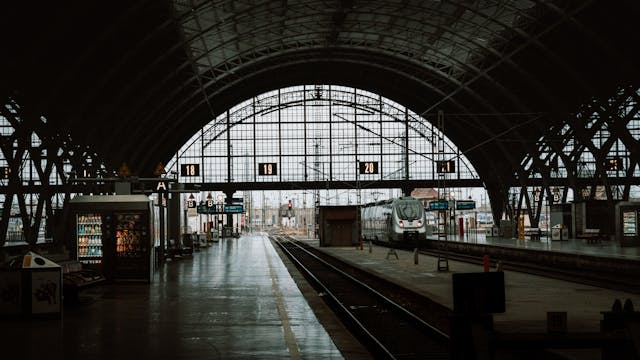
\includegraphics[width = 0.5\textwidth]{image.jpeg}
%     \caption{Cool train station}
%     \label{fig: image}
% \end{figure*}

\end{ZhChapter}
% 章節二 Chapter 2
\begin{ZhChapter}
    \chapter{Related Work}
    In the following section, we will introduce the concept of metaheuristics \cite{yang2010nature,yang2011metaheuristic} . Then, we will discuss the importance of loss functions and their role in deep learning \cite{deepLearning} models. Finally, we will explore image classification \cite{rawat2017deep} and its real-life applications.

    \section{Metaheuristic}
    Metaheuristic \cite{glover1986future} was first proposed by \citeauthor{glover1986future}. It can be regarded as a high-level procedure used to find solutions to optimization problems or other issues that conventional algorithms cannot solve. Within metaheuristics, an important concept is that these procedures must find a potentially optimal solution under reasonable computational costs or insufficient information. In this paper, we will primarily focus on nature-inspired metaheuristics \cite{yang2010nature}. In these methods, a common approach is to use a population-based strategy to find the optimal solution. Within a population, each individual typically represents a potential solution. We perform various operations on the individuals within the population to achieve our goal of approximating the optimal solution. A subset of specialized algorithms falls under population-based methods \cite{enwiki:1255593755}, commonly referred to as evolving algorithms (EAs) \cite{muhlenbein1988evolution}. Commonly used methods within EAs include genetic algorithms (GA) \cite{kumar2010genetic}, genetic programming (GP) \cite{geneticProgramming} , evolutionary programming (EP) \cite{yao1999evolutionary}, and differential evolution (DE) \cite{das2010differential}. We will briefly discuss EAs and GAs, and then we will focus primarily on GPs in the following paragraph.

    EAs can be described as algorithms inspired by the concept of "survival of the fittest \cite{paul1988selection}." These algorithms often take cues from natural evolutionary mechanisms to create algorithms that mimic animal behavior in the search for optimal solutions. Common examples include Ant Colony Optimization (ACO) \cite{dorigo2006ant}, GA, and Particle Swarm Optimization (PSO) \cite{kennedy1995particle}. In this type of algorithm, the typical approach is to initialize a population, which consists of several individuals. Each individual represents a potential optimal solution. After initializing the population, we usually set a number to represent how many generations we want this population to evolve. Before the start of each generation, a special function is used to calculate the fitness value of each individual, determining their level of excellence. Next, we perform selection, mutation, and crossover on the population. Selection involves choosing individuals based on their fitness to reproduce the next generation. Mutation generally refers to making random changes to an individual, while crossover combines the characteristics of two individuals to create the next generation. These steps are repeated until the predefined number of generations is reached, or the individuals fail to achieve the expected results, leading to a forced stop. Ultimately, the best individual in the population is obtained as the solution.

    GA is considered a type of EA, utilizing the representation of each solution in the form of chromosomes to perform selection, mutation, and crossover. GP is regarded as a special case of GAs, but due to its versatility and practicality, it is seen as a reliable solution. Unlike GAs, GP typically uses a more robust encoding method to represent chromosomes. For instance, GAs often use strings to represent chromosomes, which can present potential issues that need to be addressed, such as the priority of operations for each symbol or the validity of the equation itself. In contrast, GP usually represents chromosomes as trees, a method that can employ predefined traversal techniques to avoid these issues. It is worth noting that in GAs and GP, we can leverage their inherent ability to evolve automatically to find a reasonable optimal solution without having an in-depth understanding of the knowledge domain related to the problem we aim to solve. In the following paragraphs, we will introduce related research.

    In \cite{coreyes2022evolvingreinforcementlearningalgorithms}, \citeauthor{coreyes2022evolvingreinforcementlearningalgorithms} proposed a meta-learning reinforcement learning algorithm. They used computational graphs to represent algorithms. By doing so, algorithms could be identified, calculated, and optimized through Reinforcement Learning (RL) \cite{kaelbling1996reinforcement}. Notably, in this study, algorithms were represented as directed acyclic graphs (DAG) \cite{thost2021directedacyclicgraphneural} of nodes. Within the DAG , all nodes were classified into three categories: input nodes, parameter nodes, and operation nodes. Once the algorithms were represented as DAGs, they could be placed into RL for training and evaluation. In this proposed algorithm, they employed the concept of regularized evolution \cite{real2019regularized} to evolve a population formed by several randomized and known algorithms. The method was as follows: initialize the population with algorithms, evaluate each algorithm in the population and record their performance, then in a loop, repeatedly use a sample tournament \cite{goldberg1991comparative} to select algorithms, perform mutations on the algorithms by the mutator they designed, and evaluate them again until the loop ends. During the evaluation process, they trained and assessed the algorithms using RL, continuously testing the performance of each algorithm in different training environments. They also utilized normalized training performance to avoid numerical biases caused by varying environments. Through this approach, the study successfully created two algorithms, named DQNClipped and DQNReg, which outperformed classical control tasks.

    In \cite{akhmedova2024generationlossfunctionimage}, \citeauthor{akhmedova2024generationlossfunctionimage} proposed a genetic programming-based method to find a better function for the image classification training task. They encoded the loss functions into trees, with each tree considered an individual. All individuals were aggregated into a population. In this study, the population was evolved across multiple generations. Before the start of each generation, all individuals were evaluated. Each individual had a probability of undergoing crossover with an individual from a special external archive to create a new individual; otherwise, it would perform the crossover with another individual. Following this, two probabilistic decisions were made. If successful, the new individual could perform subtree mutation or one-point mutation, respectively. At the end of each generation, the fitness value of all individuals was re-evaluated. A certain number of low-scoring individuals were eliminated to the special external archive mentioned earlier, maintaining the stability of the population's size. After these steps, a new generation began, continuing until a predefined number of generations was reached.  By employing this method, this study successfully evolved an outstanding individual within the population, creating a function that could train an image classification model more effectively compared to Cross Entropy (CE) \cite{zhang2018generalized}.

    \section{Loss Function}

    \subsection{Deep Learning Model}
    In recent years, due to the significant increase in the computational speed of GPUs, training deep learning models to solve a wide variety of problems has become widely regarded as a feasible and popular solution. The process of training a deep learning model is often divided into several steps: collecting the data needed to train the model, and adding ground truth values to the data according to the model's requirements. Ground truth can be thought of as the ideal answers we hope to achieve after the model's computation. Once the data collection is complete, these data sets are collectively referred to as the dataset. Typically, the dataset is divided into training sets, validation sets, and testing sets. Data from the training set are used to train the model, the validation set is used to evaluate the model's effectiveness after each training loop, and the testing set is used to calculate the model's final score and determine whether the model successfully achieves its designed purpose. It is worth noting that the testing set data should not be seen during training and validation phases. After dividing the dataset, we decide on the model's architecture. Common architectures include Fully Connected Networks (FCN) \cite{iliadis2018deep} and Convolutional Neural Networks (CNN) \cite{wu2017introduction}, etc. Then the training process can begin. During training, we compare the model's output with the ground truth of the training data and use a loss function to calculate the difference between the output and the ground truth. This guides the adjustment of the model's parameters. Therefore, the loss function significantly determines the effectiveness of model training, and this aspect will be explained further later. After adjusting the model, the next round of training begins, continuing until the training is deemed ineffective or a predetermined maximum number of iterations is reached.
    \subsection{Importance of Loss Function}
    In \cite{gonzalez2020improvedtrainingspeedaccuracy}, a loss function meet genetic programming is proposed ....
    \section{Image Classification}

    % \subsection{}
    % 定義定義定義定義定義定義\cite{latex2e},定義定義定義定義,定義定義定義定義定義定義定義定義定義定義,定義定義。

    % \begin{table*}[htbp]
    %     \centering
    %     \caption{表格範例標題} \label{tab: complexity}
    %     \makebox[\linewidth][c]{
    %     \renewcommand\arraystretch{1.2}{
    %         \begin{tabular}{| l | c  c  c  c |}
    %         \hline
    %         Protocol & $P$ & $CS_1$ & $CS_2$ & $RG$ \\
    %         \hline
    %         MSSMul & $O(1)$, $O(1)$, N/A & $O(n-t)$, $O(n)$, $O(1)$ & $O(n-t)$, $O(n)$, N/A & $O(1)$, $O(n)$, $O(n)$ \\
    %         SC & $O(1)$, $O(1)$, N/A & $O(n-t)$, $O(n)$, $O(1)$ & $O(n-t)$, $O(n)$, N/A & $O(1)$, $O(n)$, $O(n)$ \\
    %         \hline 
    %         \end {tabular}
    %     }}
    % \end {table*}

    % \section{模型說明(小標)}

    % 說明說明說明說明,說明說明說明說明說明說明說明說明說明說明說明說明,說明說明說明說明說明說明說明說明。

    % \begin{figure*}[htbp]
    %     \centering
    %     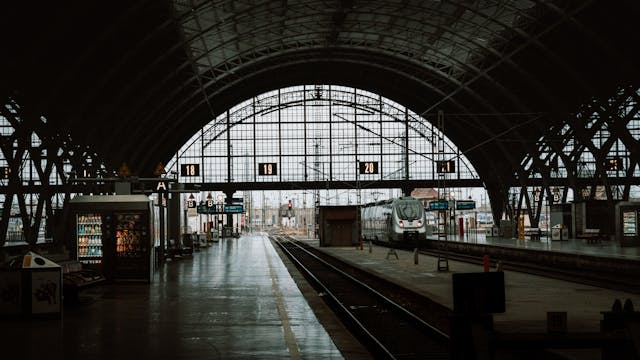
\includegraphics[width = 0.5\textwidth]{image.jpeg}
    %     \caption{Cool train station}
    %     \label{fig: image}
    % \end{figure*}

\end{ZhChapter}
% 新增你自己的章節... Add chapters here

% 參考文獻,請在段落上隨意註解,你同時需要 reference.bib
%\addcontentsline{toc}{chapter}{References}
%\printbibliography[title=References]




\end{document}
